\documentclass[authoryear,3p]{elsarticle}
\journal{Remote Sensing of Environment}
\bibliographystyle{model5-names}\biboptions{authoryear}

\usepackage{adjustbox}
\usepackage{array}
\usepackage{booktabs}
\usepackage{graphicx}

\renewcommand\thetable{S\arabic{table}}
\renewcommand\thefigure{S\arabic{figure}}

\begin{document}
\begin{table}[h!]
\begin{center}
\begin{adjustbox}{max width=12cm}
\begin{tabular}{m{12cm}l}
\toprule
\multicolumn{1}{l}{Category \& data source}&\multicolumn{1}{c}{Covariate}\tabularnewline
\midrule
Location (3, intrinsic)&
\begin{tabular}{@{}l@{}}longitude\tabularnewline
latitude\tabularnewline
absolute latitude
\end{tabular}\tabularnewline
\midrule
Vegetation indices (22, derived from PROBA-V 100m top-of-canopy reflectance v1.02 \citep{dierckx2014probav})&
\begin{tabular}{@{}l@{}}
minimum NDVI\tabularnewline
maximum NDVI\tabularnewline
median NDMI\tabularnewline
NDMI yearly IQR\tabularnewline
NDMI March-May IQR\tabularnewline
NDMI June-August IQR\tabularnewline
NDMI September-November IQR\tabularnewline
NDMI December-February IQR\tabularnewline
OSAVI March-May IQR\tabularnewline
OSAVI June-August IQR\tabularnewline
OSAVI September-November IQR\tabularnewline
OSAVI December-February IQR\tabularnewline
EVI March-May IQR\tabularnewline
EVI June-August IQR\tabularnewline
EVI September-November IQR\tabularnewline
EVI December-February IQR\tabularnewline
median NIRv\tabularnewline
NIRv yearly IQR\tabularnewline
NIRv March-May IQR\tabularnewline
NIRv June-August IQR\tabularnewline
NIRv September-November IQR\tabularnewline
NIRv December-February IQR
\end{tabular}\tabularnewline
\midrule
Temporal metrics (9, derived from a harmonic model over time series of PROBA-V 100m top-of-canopy reflectance v1.02 \citep{dierckx2014probav})&
\begin{tabular}{@{}l@{}}
NDVI order 1 cosine\tabularnewline
NDVI order 1 sine\tabularnewline
NDVI order 2 cosine\tabularnewline
NDVI order 2 sine\tabularnewline
NDVI trend coefficient\tabularnewline
NDVI order 1 phase\tabularnewline
NDVI order 1 amplitude\tabularnewline
NDVI order 2 phase\tabularnewline
NDVI order 2 amplitude
\end{tabular}\tabularnewline
\midrule
Terrain (4, ASTER GDEM V003 \citep{ASTGTM003})&
\begin{tabular}{@{}l@{}}
elevation\tabularnewline
slope (log-transformed)\tabularnewline
aspect\tabularnewline
terrain position index
\end{tabular}\tabularnewline
\midrule
Climate (21, WorldClim 2.0 \citep{worldclim2})&
\begin{tabular}{@{}l@{}}
January precipitation (log)\tabularnewline
April precipitation (log)\tabularnewline
July precipitation (log)\tabularnewline
October precipitation (log)\tabularnewline
January solar irradiance\tabularnewline
July solar irradiance\tabularnewline
mean temperature\tabularnewline
temperature monthly range\tabularnewline
isothermality\tabularnewline
temperature annual range\tabularnewline
annual precipitation (log)\tabularnewline
temperature seasonality\tabularnewline
minimum solar irradiance\tabularnewline
maximum solar irradiance\tabularnewline
mean solar irradiance\tabularnewline
mean windspeed\tabularnewline
mean water vapour pressure\tabularnewline
coldest month precipitation (log)\tabularnewline
warmest month precipitation (log)\tabularnewline
wettest month solar irradiance\tabularnewline
driest month solar irradiance
\end{tabular}\tabularnewline
\midrule
Soil (8, SoilGrids \citep{hengl_soilgrids250m_2017})&
\begin{tabular}{@{}l@{}}
soil available water\tabularnewline
soil bulk density\tabularnewline
soil cation exchange capacity (log)\tabularnewline
soil clay fraction\tabularnewline
soil coarse fragments (log)\tabularnewline
soil pH\tabularnewline
soil sand fraction\tabularnewline
soil water wilting point
\end{tabular}\tabularnewline
\bottomrule
\end{tabular}
\end{adjustbox}
\caption{List of covariates used as input for the models tested in this study, and their data sources.}
\label{tab-inputdata}
\end{center}
\end{table}

\begin{figure}
    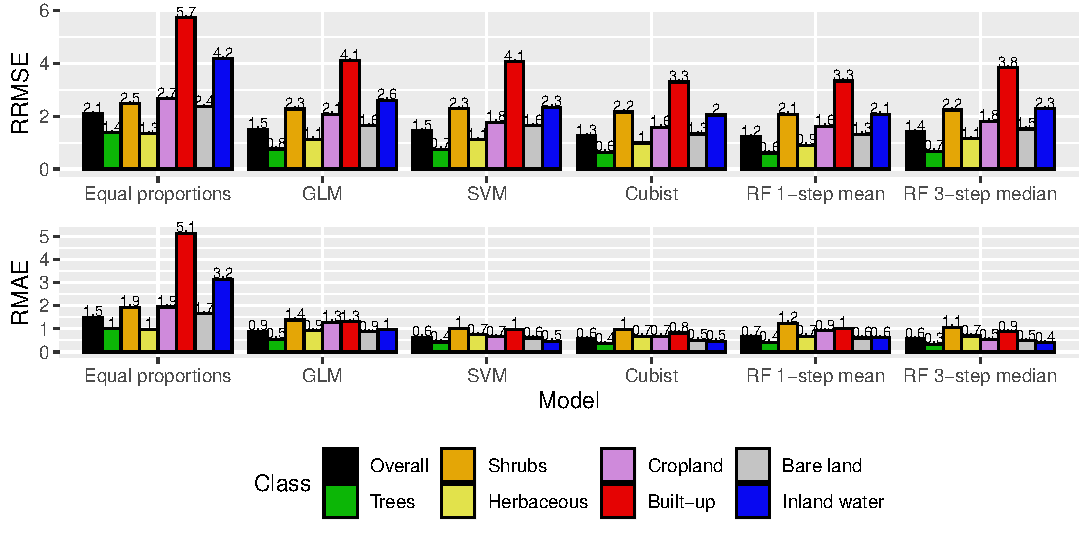
\includegraphics[width=\textwidth]{article-figures/barplots/2020-11-02-model-comparison-bar}
    \caption{Comparison of relative RMSE (top) and relative MAE (bottom) per class of the best performing models in their category, and the equal proportions solution as a reference.}
    \label{fig-models}
\end{figure}

\begin{figure}
    \centering
    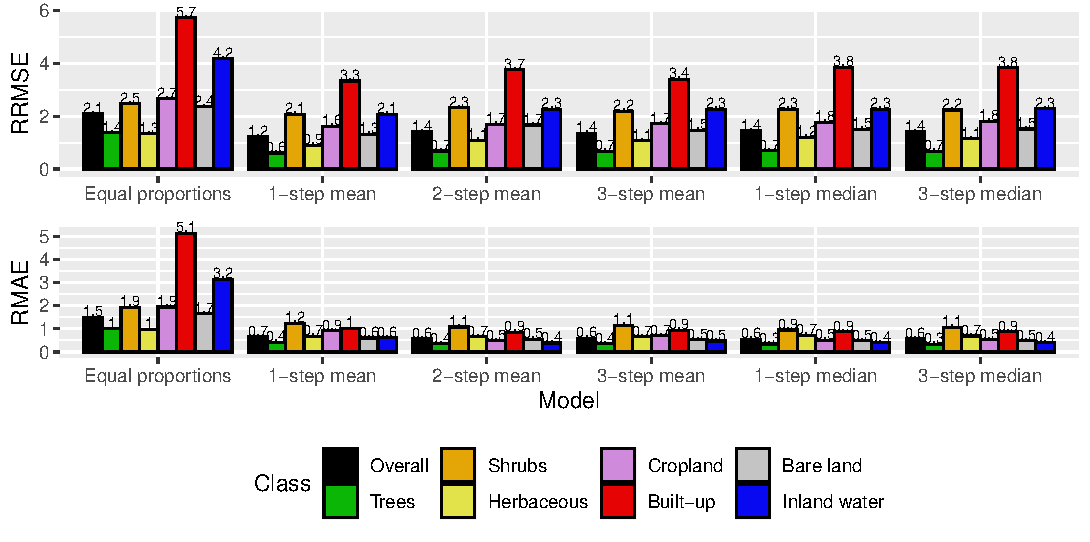
\includegraphics[width=\textwidth]{article-figures/barplots/2020-11-02-rf-comparison-bar}
    \caption{Comparison of relative accuracy metrics of RF regression models (equal proportion model shown as a reference). 1-step models use no adjustment for zero inflation, 2-step models perform classification on zeroes and regression for non-zeroes, 3-step models perform a classification into pure and non-pure pixels, and then a regression or classification based on that. Mean and median are the tree vote summary statistics.}
    \label{fig-randomforest}
\end{figure}

\bibliography{article-bib}
\end{document}
